\section{Basic Concepts}

\subsection{Definitions}

\begin{definition}[Target point]
    Target point is the point at which a negotiator would like to conclude
    negotiations, i.e. his aspired goal. The target point is often referred to
    as the 'negotiator's aspiration'.
\end{definition}

\begin{definition}[Resistance point]
    Resistance point is a negotiator's bottom line - the most he will pay as a
    buyer (for a seller, it is the smallest amount she/he will settle for).
    The resistance point is often referred to as the 'reservation price'.
\end{definition}

\begin{definition}[Starting point]
    Starting point (or asking price, initial offer) is the initial price set by the
    seller/buyer.
\end{definition}

\begin{definition}[ZOPA]
    Zone of potential agreement (ZOPA) (bargaining range, settlement range)
    is the spread between the resistance points of the negotiating parties.
\end{definition}

\subsection{Distributive negotiation}

It is a negotiation in a competitive way over one issue, a win-lose situation,
such as haggling over a price in a bazar.

\begin{example}[Selling/Buying a flat]
\end{example}

\begin{figure}[H]
    \centering
    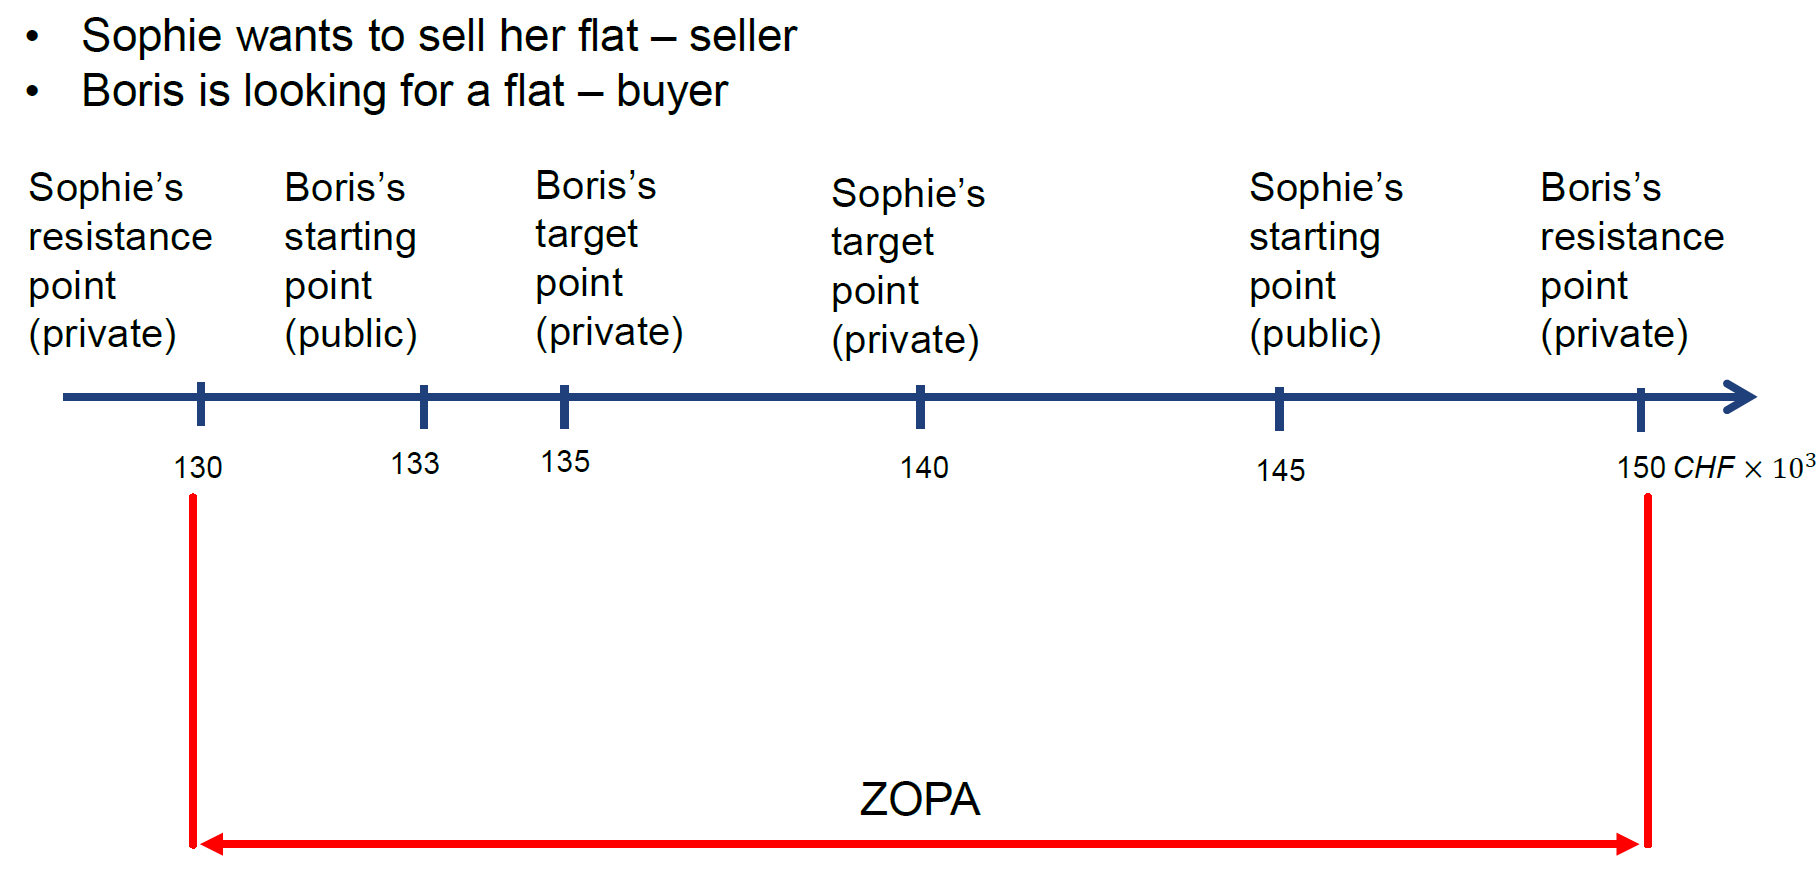
\includegraphics[width=0.5\textwidth]{Pictures/Distributive_negotiation_example_1_1.png}
    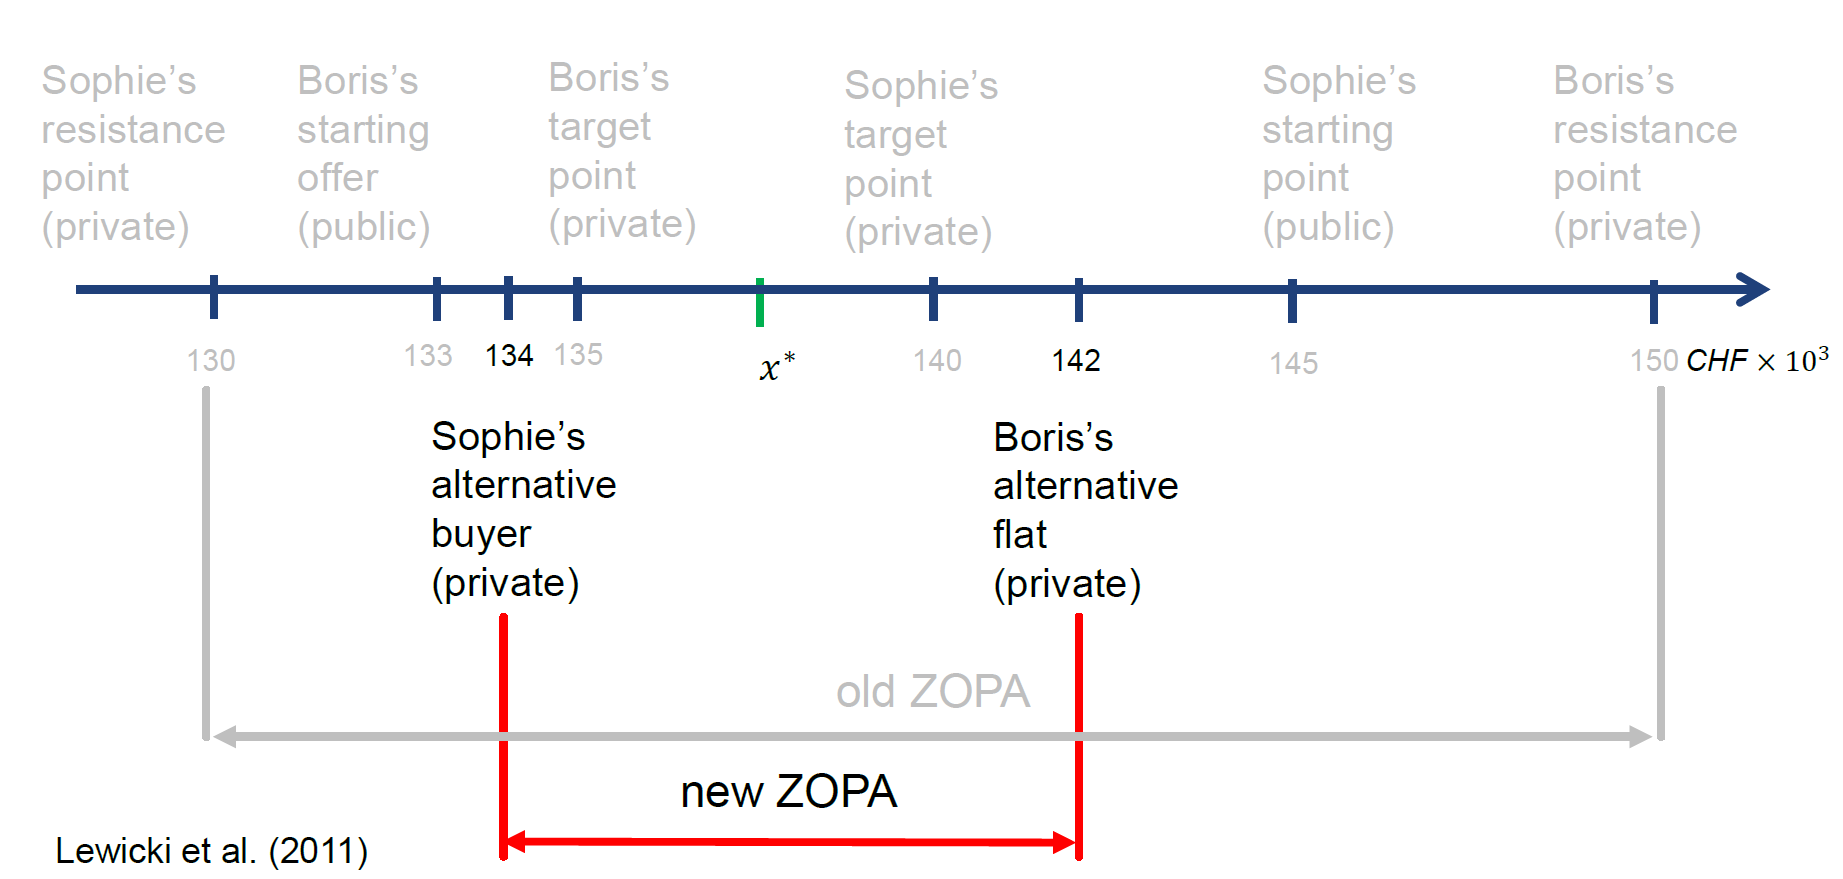
\includegraphics[width=0.5\textwidth]{Pictures/Distributive_negotiation_example_1_2.png}
    \caption{ZOPA without and with alternatives}
\end{figure}

\paragraph{Formal model}

Negotiation:

\begin{itemize}
    \item $b_R$: buyer's resistance point (i.e. the maximum price buyer would agree to pay)
    \item $s_R$: seller's resistance point (i.e. the minimum price seller would settle for)
    \item $x^\ast$: final price
    \item Seller's surplus: $\Delta_S = x^\ast - s_R$
    \item Buyer's surplus: $\Delta_B = b_R - x^\ast$
    \item The total surplus from the deal: $\Delta= \Delta_S + \Delta_B = b_R - s_R$
    \item Note: If $\Delta \geq 0$ there is a ZOPA. If $\Delta < 0$ ther is no ZOPA.
\end{itemize}

\begin{figure}[h]
    \centering
    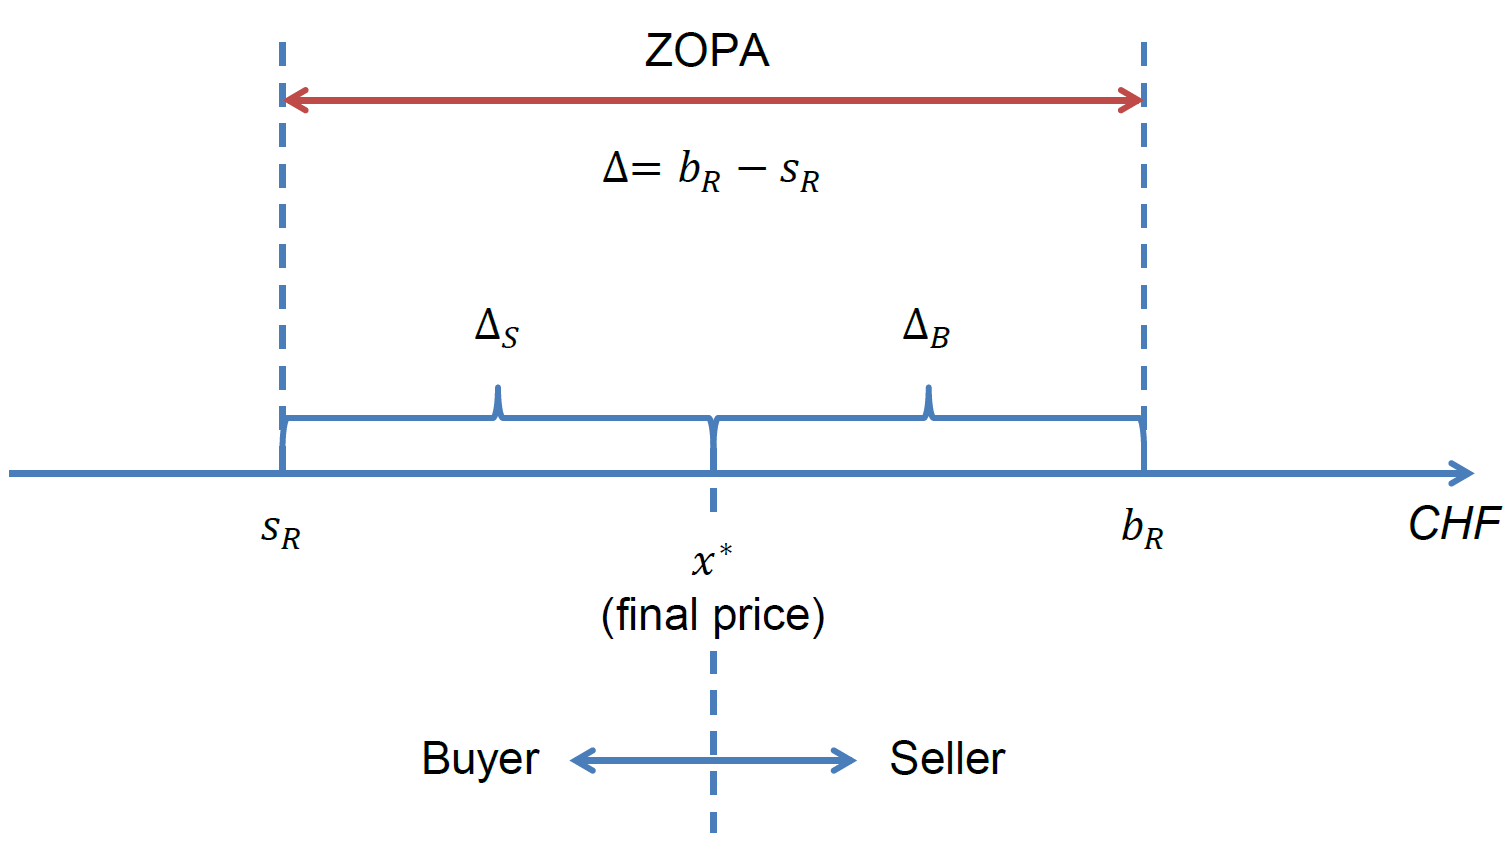
\includegraphics[width=0.5\textwidth]{Pictures/Seller_Buyer_model.png}
    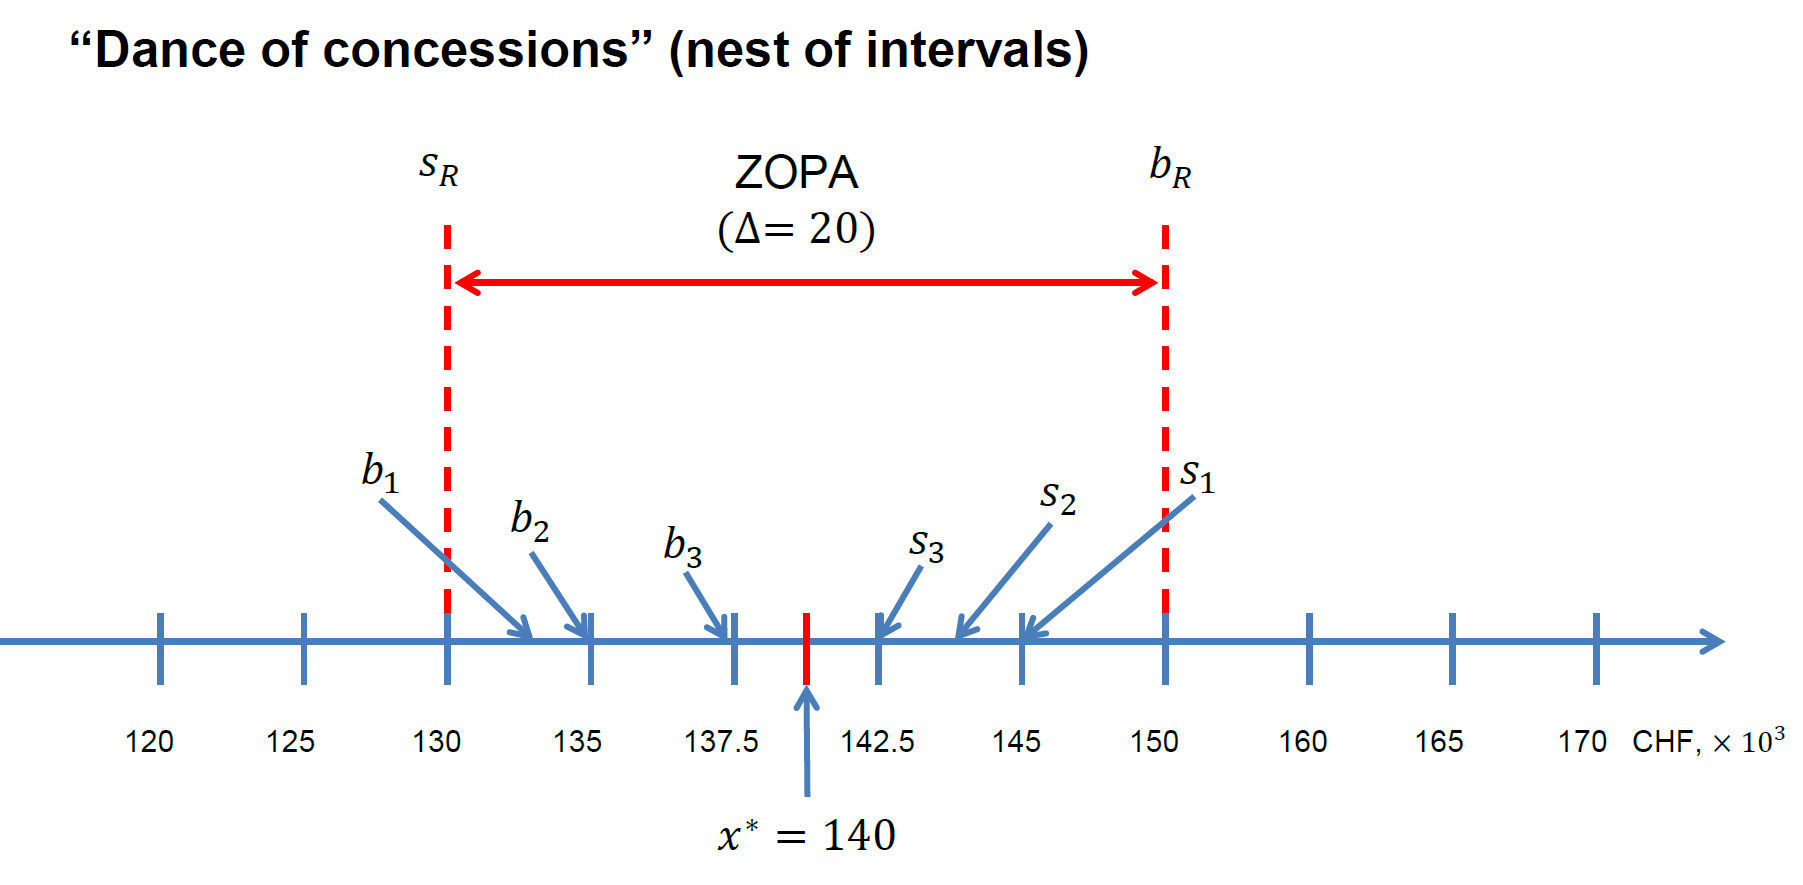
\includegraphics[width=0.5\textwidth]{Pictures/Dance_of_concessions.png}
\end{figure}

\paragraph{Comments}
\begin{itemize}
    \item Achieve the most preferable outcome within the bargaining range
    \item Subjective assessment/perception of the deal
    \item By making high offers and small concessions you can attempt to review the
        resistance points
    \item It is important that people feel as if they got the best possible deal.
\end{itemize}

\subsection{Integrative negotiation}

It is a negotiation that can look for win-win solutions or problem solving
in order to achieve a mutual gain.

\begin{example}[Acquisition of a company]
    \begin{itemize}
        \item A big international corporation (Firm B) wants to make a friendly
            acquisition of one of its suppliers, the small company (Firm S)
        \item Both agree that Firm S would be more valuable as a part of Firm B.
        \item Despite this agreement, they are unable to complete the acquisition.
        \item Firm B offers CHF 13.5 million for Firm S, but firm S insists on CHF
            16.5 million.
        \item Efforts to find a compromise fail: neither side finds 15 CHF acceptable.
    \end{itemize}
\end{example}

\begin{figure}[h]
    \centering
    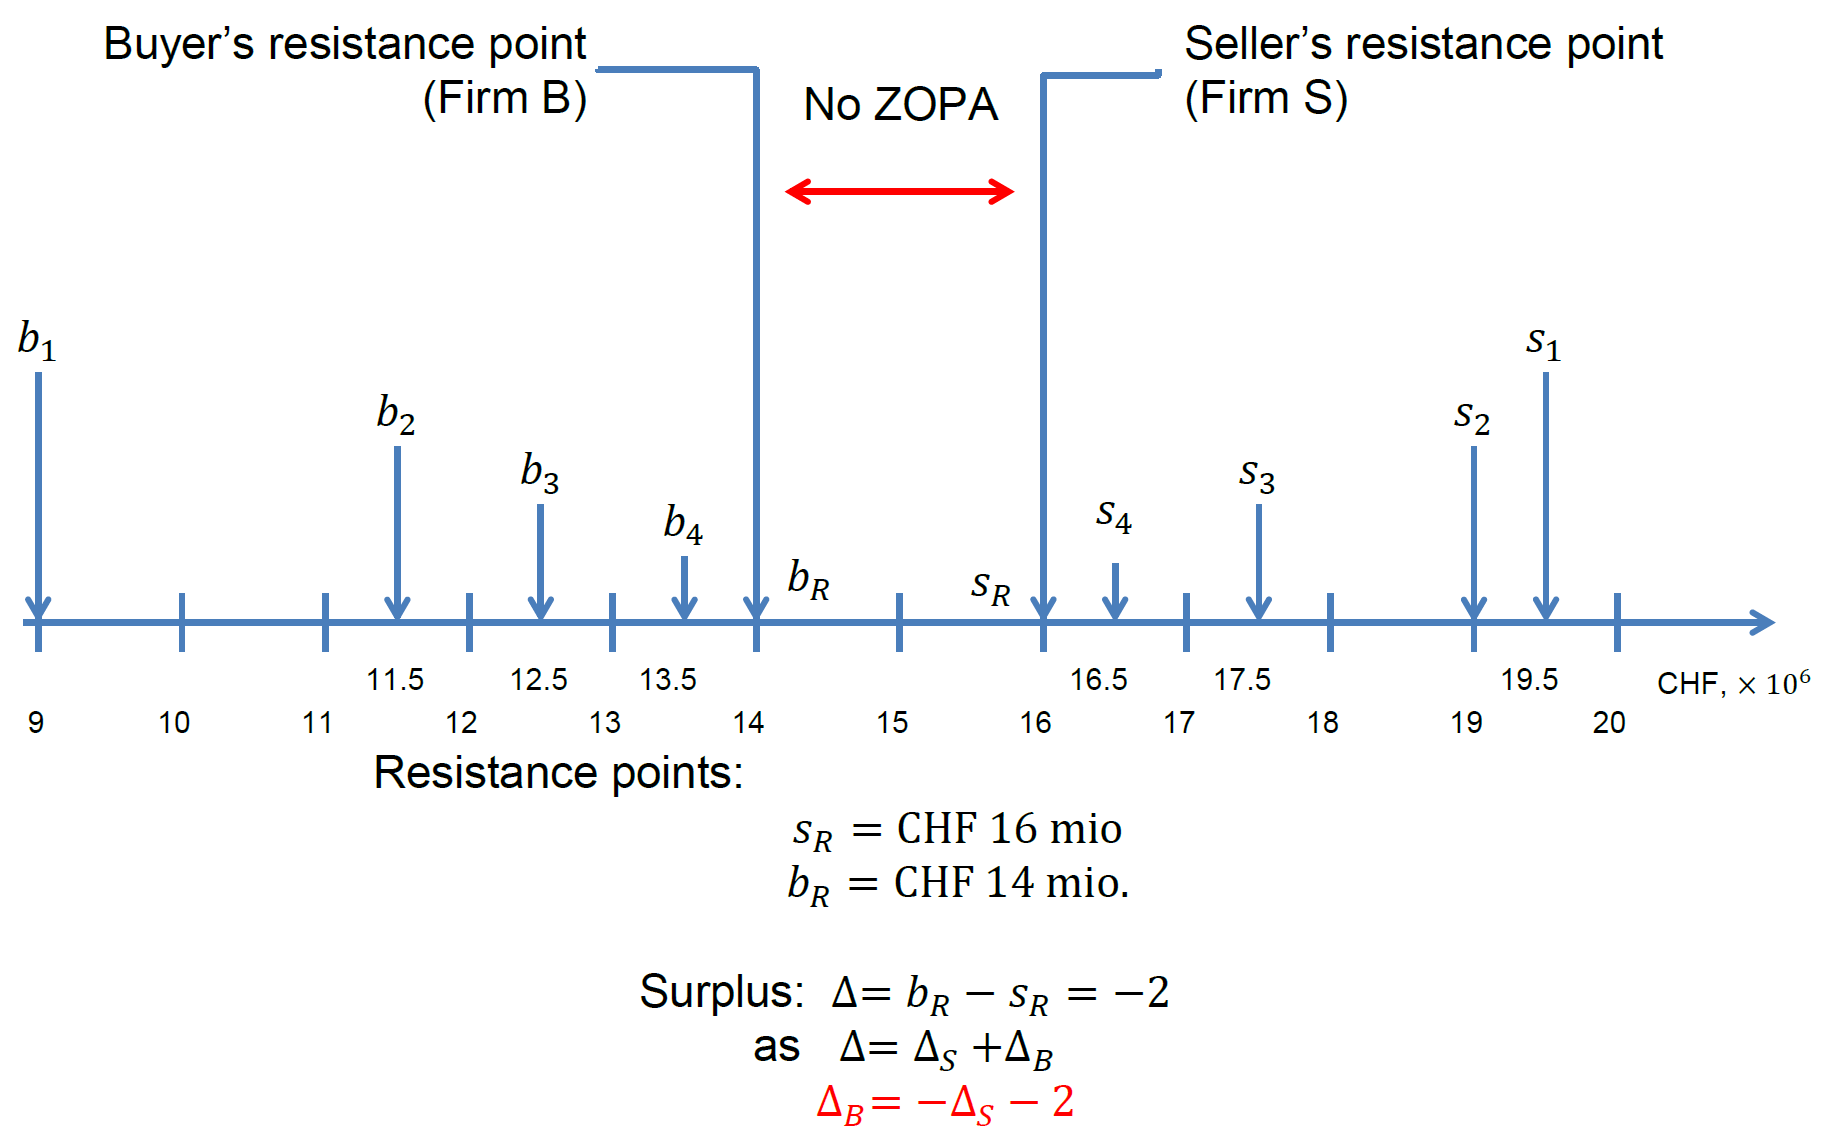
\includegraphics[width=0.5\textwidth]{Pictures/Example_2.png}
\end{figure}

\begin{itemize}
    \item Both firms do some research and realize that the two have different views
        of the value of a new high-tech, high-risk Division D.
    \item Firm B considers Divition D worth only 1 million CHF (of the 14 mio resistance point)
        whilt firm S truly believes in the viability of the new products under development
        and has valued this division at 6 million CHF (of the 16 mio resistance point)
    \item When the parties realize this, they can trade-off on this underlying issue,
        in order to find an agreement: Firm B acquires Firm S for 12 million CHF,
        but the owners of the Firm S retain control of Dividion D.
\end{itemize}

\paragraph{Formal model}

Different valuations of Divition D:
\begin{itemize}
    \item Firm S values it at CHF 6 mio
    \item Firm B values it at CHF 1 mio
\end{itemize}
New resistance points:
\begin{align*}
    s_R &= \text{CHF } 10 \text{ mio } (= 16-6)
    \\
    b_R &= \text{CHF } 13 \text{ mio } (= 14-1)
\end{align*}
Surplus: $\Delta = b_R - s_R = 13-10 = +3$ as $\Delta = \Delta_S + \Delta_B$.
For any price $x^\ast$ the buyer's and seller's surplusses are related to
$\Delta_B = - \Delta_S + 3$. A fair price could be in the middle of 10 and 13 mio.
$x^\ast = 11.5$ mio.

\begin{figure}[h]
    \centering
    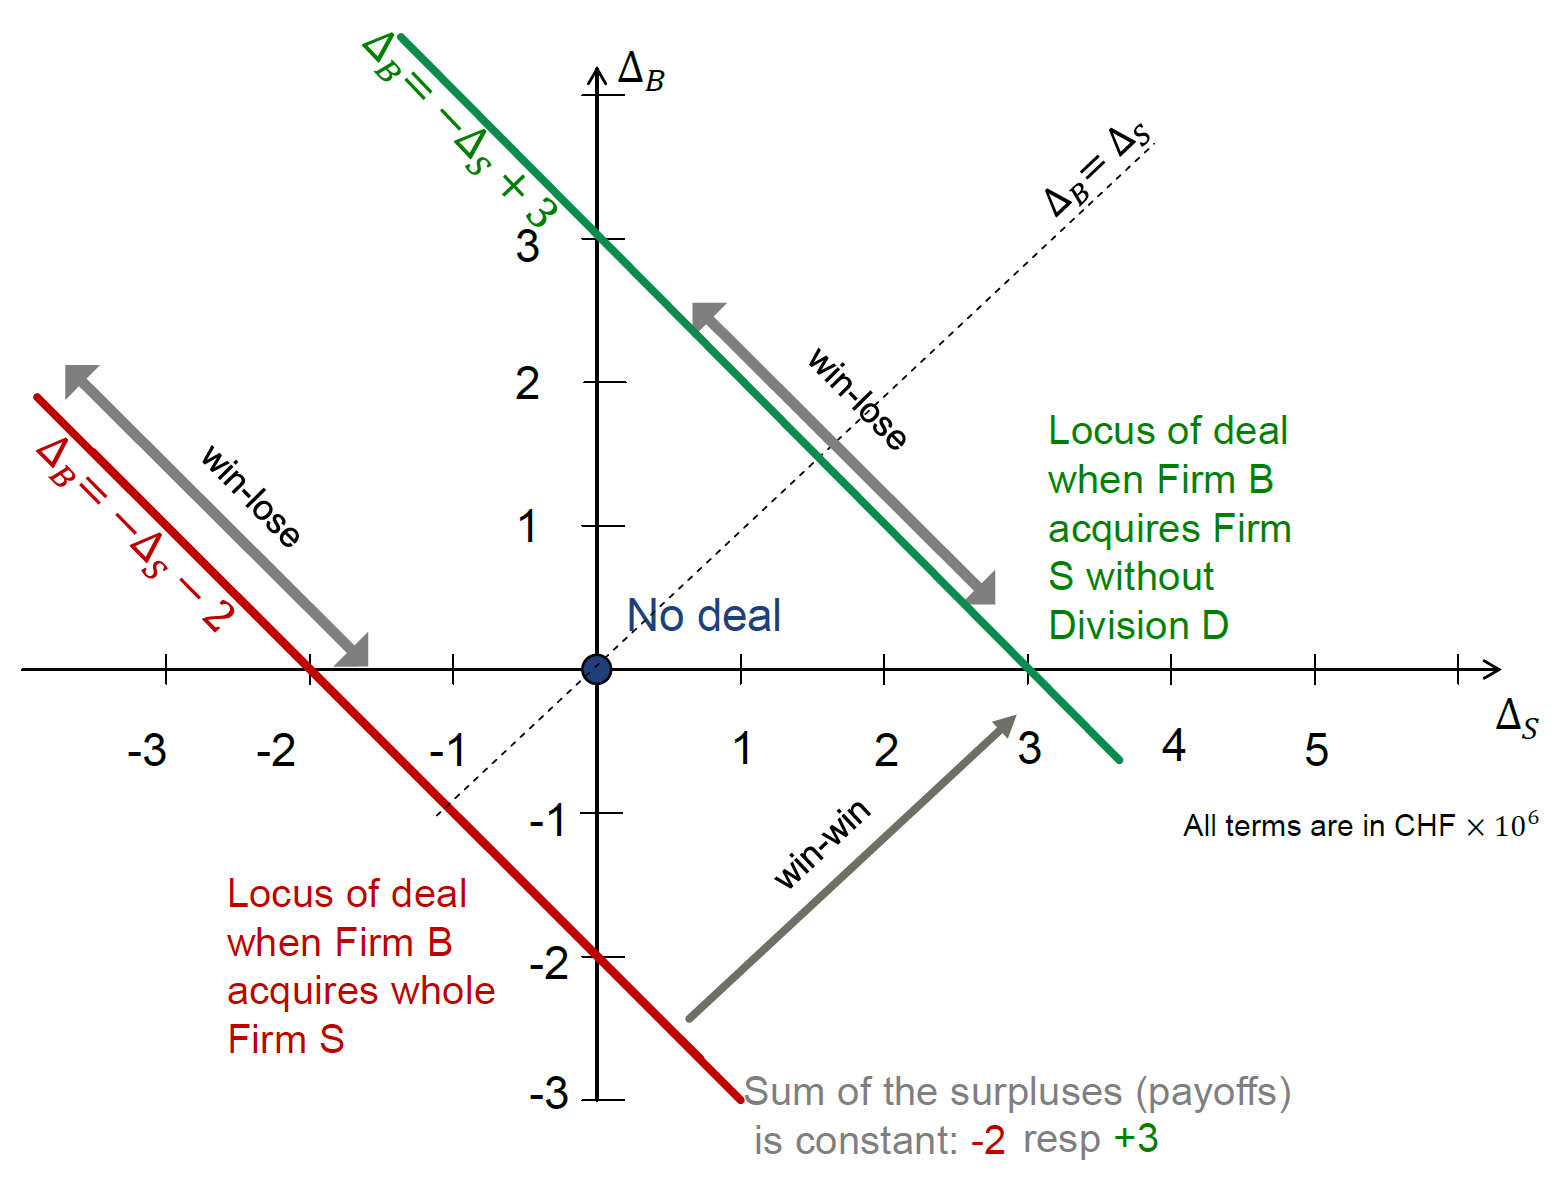
\includegraphics[width=0.5\textwidth]{Pictures/Integrative_negotiation_plot.png}
\end{figure}

\paragraph{Steps in integrative negotiation}

\begin{enumerate}
    \item Sides need to agree on what the problem is
    \item What are the interests behind the positions
    \item Generate alternative solutions
        \begin{itemize}
            \item Redefine the problem (Exapmle 3)
                \begin{itemize}
                    \item Expand pie
                    \item Logroll
                    \item Offer compensation in other area
                    \item minimize costs
                    \item Bridge
                \end{itemize}
            \item Generate solutions for the given problem
        \end{itemize}
    \item Make a list of solutions
    \item Prioritize options and reduce the list
    \item Select a solution
\end{enumerate}

\begin{example}[Generaet alternative solutions]
    \begin{itemize}
        \item The Problem: What will a husband and wife do with 2 weeks of vacation?
        \item Interests:
            \begin{itemize}
                \item She wants: mountains, hiking, and other outdoor activities, rustic cabin
                \item He wants: beach, swimming, and night life, fancy hotel
            \end{itemize}
        \item Generate alternative solution:
            \begin{itemize}
                \item Expand pie: make 4 weeks - 2 weeks mountains; 2 weeks beach
                \item Logrolling: (1) fancy hotel in the mountains or (2) rustic hotel on the beach
                \item Compensation in other area: he pays her a ski equipment, she accepts to go the beach
                \item Minimize cost: he accepts to take a beach house away from the big hotels
                \item Bridge: they choose a place that offres hiking, mountains, swimming, beaches and night life
            \end{itemize}
    \end{itemize}
\end{example}

\paragraph{Comments}
Additional important elements:
\begin{itemize}
    \item Fairnes and other intangibles
        \begin{itemize}
            \item Outcome is equally shared ("divide it down the middle")
            \item Outcome is devided based on equity
            \item Outcome is divided based on needs
        \end{itemize}
    \item Emotional escalation
    \item Difference in risk preferences, expectations, time preferences
    \item "Nothing is agreed until everything is agreed!"
\end{itemize}

\subsection{Best practices}

Lewicki: Ten best practices

\begin{enumerate}
    \item Be prepared
    \item Diagnose the fundamental structure of the negotiation
    \item Work the BATNA (Best alternative to the negotiated agreement)
    \item Be willing to walk away
    \item Master the paradoxes
    \item Remember the intangibles
    \item Actively manage colitions
    \item Savor and protect your reputation
    \item Remember that rationality and fairness are relative
    \item Continue to learn from experience
\end{enumerate}